\documentclass[C]{beamer}
\usepackage[utf8]{inputenc}
\usepackage[T1]{fontenc}
\usepackage[francais]{babel}
\usepackage{hyperref}
\usepackage{ragged2e}
\justifying
\usepackage{multimedia}

\setbeamercolor{background canvas}{bg=yellow!10!white}

\usetheme{Warsaw}
\title{Thème 1~: Du développement au développement durable}

\author{M. Lavastrou}
\institute{Classes de seconde -- Lycée Jean Lurçat}
\date{Année scolaire 2016-2017}
%temps 7-8h
\begin{document}
	\begin{frame}
	\titlepage
	\end{frame}
	
	\section*{Introduction}
	\subsection*{Définition}
	\begin{frame}
	\frametitle{Introduction~: définitions}
	\begin{itemize}
	\item \textbf{Qu'est-ce que le développement}~?\\
\pause
		\begin{itemize}
		\item C'est un accroissement des richesses associé à l'amélioration des conditions de vie d'une population sur un territoire.
		\end{itemize}
	\item \textbf{Qu'est-ce que le développement durable}~?\\
\pause
		\begin{itemize}
		\item le \textbf{rapport Bruntland} a défini, en 1987, le concept de développement durable «~comme un développement qui répond aux besoins des générations présente sans compromettre la capacité des générations futures à satisfaire les leurs. Au strict minimum, cela signifie de ne pas mettre en danger les systèmes naturels nécessaires à notre vie~: l'eau, l'air, les sols et les \^etres vivants~».
		\end{itemize}
	\end{itemize}
	\end{frame}
	
	\begin{frame}
	\frametitle{Introduction~: le développement durable, ses implications}
	\begin{itemize}
	\item le concept de développement durable implique donc de concilier l'environnement et un développement économique qui impliquent une gestion raisonnée des ressources naturelles afin d'assurer la survie de la planète
	\item le développement durable repose sur trois piliers~: 
		\begin{itemize}
		\item il doit \^etre écologiquement reproductible\\
\pause
		\item économiquement viable\\
\pause
		\item socialement équitable
		\end{itemize}
	\end{itemize}
=> cela induit de la part de l'Homme une responsabilité dans le temps (futur) et dans l'espace (la planète) vis-à-vis de la nature
	\end{frame}
	
	\subsection*{\'Eléments de contexte}
	\begin{frame}
	\frametitle{Introduction~: élément de contexte}
	Aujourd'hui la Terre comporte 7 milliards d'individus et plus de 9 milliards (9,6 milliards) sont attendus en 2050. Déjà, tout le monde ne mange pas à sa faim, ou n'a pas accès à l'école, à l'information, à la santé, ou encore au logement. Par conséquent, on ne peut que constater des inégalités fortes et nombreuses à l'échelle mondiale comme au niveau local. Un des enjeux du développement (et du développement durable) est de limiter ces inégalités tout en faisant face aux besoins croissants d'une population en perpétuelle augmentation.
	\end{frame}
	
	\subsection*{Problématique \& Plan}
	\begin{frame}
	\frametitle{Introduction~: Problématique}
	\begin{enumerate}
	\item Comment faire face aux besoins d'une humanité toujours plus nombreuse~?\\
\pause
	\item Le développement durable est-il une réponse aux problèmes du monde~?
	\end{enumerate}
	\end{frame}
	
	\begin{frame}
	\frametitle{Introduction~: Plan}
	\begin{enumerate}
	\item Des inégalités de développement
	\item De nouveaux besoins pour une humanité de plus de 9 milliards en 2050
	\item Vers des modes durables de développement~?
	\end{enumerate}
	\end{frame}
	
	\section*{I -- Des inégalités de développement}
	\subsection*{A -- comment mesurer les inégalités~?}
	\begin{frame}
	\frametitle{I -- Des inégalités de développement\\ A -- comment mesurer les inégalités~?}
	\begin{center}
	\textbf{D'après vous, comment peut-on mesurer les inégalités de développement dans le monde~? Entre d'autres termes, avec quels indicateurs, peut-on mesurer ce déséquilibre de développement~?}\\
\pause
	\end{center}
	\begin{itemize}
	\item le \textbf{PIB}~: Produit Intérieur Brut, cet indicateur mesure la richesse et plus particulièrement le niveau de vie dans un pays donné. Le PIB par habitant a augmenté de 50\% en 20 ans, cependant les inégalités demeurent très fortes~: dans le monde 5\% des plus riches reçoivent le tiers du revenu mondial et 5\% des plus pauvres se contentent de 0,2\%.
	\end{itemize}
	\end{frame}
	
%	\begin{frame}
%	\frametitle{I -- Des inégalités de développement\\ A -- Comment mesurer les inégalités~?}
%	\end{frame}
	
%	\begin{frame}
%	\frametitle{I -- Des inégalités de développement\\ A -- Comment mesurer les inégalités~?}
%	\begin{center}
%	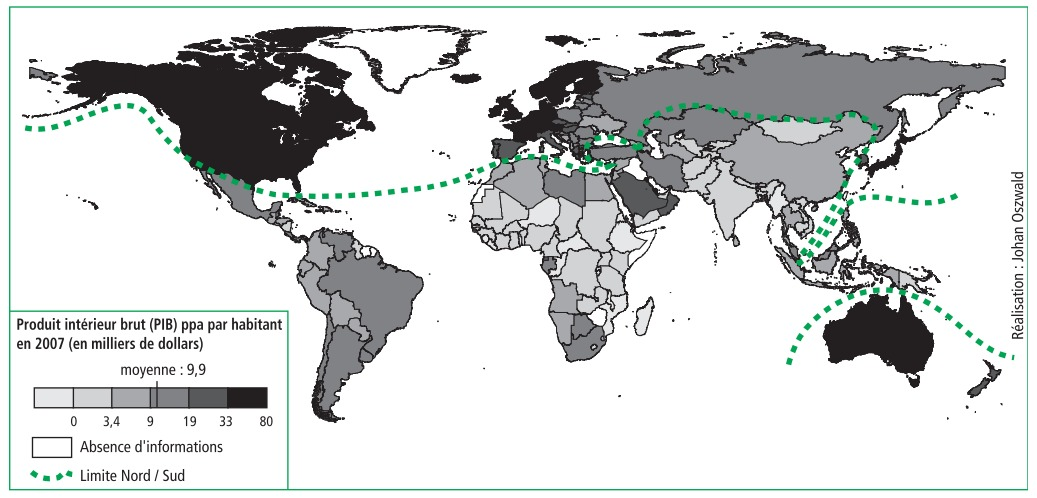
\includegraphics[height=5.5cm]{images/carte_1_01.jpg}
%	\end{center}
%	\end{frame}
	
	\begin{frame}
	\frametitle{I -- Des inégalités de développement\\ A -- comment mesurer les inégalités~?}
	\begin{itemize}
	\item l'\textbf{IDH}~: l'Indice de Développement Humain. La pauvreté n'est pas seulement liée à l'argent, elle se manifeste par une espérance de vie plus faible, un bas niveau d'éducation, etc. Ainsi, 2 milliards d'hommes ont une ration alimentaire quotidienne incomplète, par conséquent 2 milliards d'êtres humains ne mangent pas leur faim, des maladies comme le sida (VIH) et le paludisme font des ravages et diminuent l'espérance de vie faute de traitement, enfin, \textbf{770 millions d'adultes sont analphabètes} dans le monde.
	\item Voir par exemple la carte 2 «~L'espérance de vie dans le monde en 2012~», p.12
	\end{itemize}
	\end{frame}
	
%	\begin{frame}
%	\frametitle{I -- Des inégalités de développement\\ A -- Comment mesurer les inégalités~?}
%	\begin{center}
%	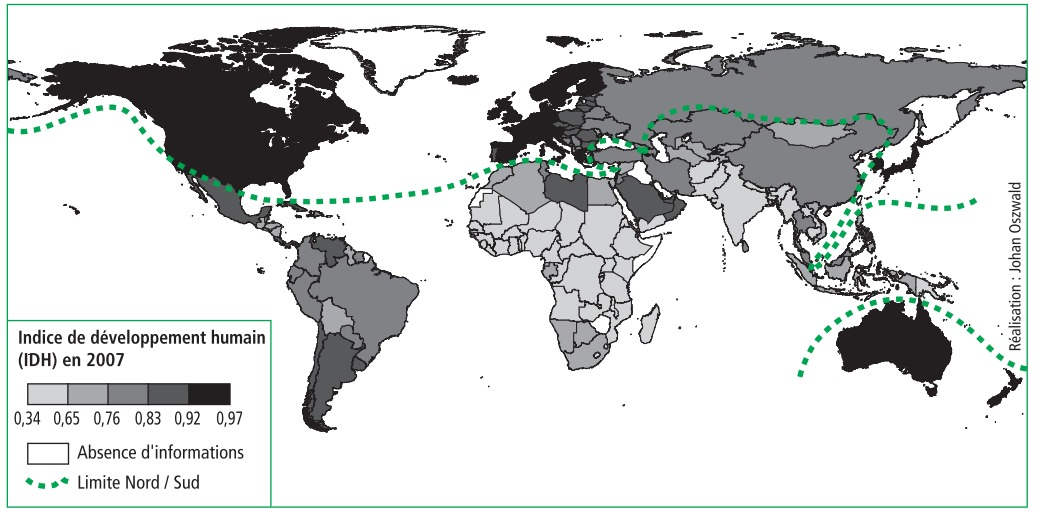
\includegraphics[height=5.5cm]{images/carte_1_02.jpg}
%	\end{center}
%	\end{frame}
	
	\begin{frame}
	\frametitle{I -- Des inégalités de développement\\ A -- comment mesurer les inégalités~?}
	\begin{itemize}
	\item l'\textbf{IPH}~: Indicateur de Pauvreté Humaine est un indice permettant de caractériser le niveau de pauvreté d'un pays. La pauvreté affecte les pays du \textbf{Sud}, en particulier l'\textbf{Afrique subsaharienne et l'Asie du Sud} où les pays les plus pauvres sont nommés PMA (Pays les moins avancés). Cependant, des pays du Sud peuvent avoir un fort PIB comme les \textbf{pays pétroliers} (Arabie Saoudite). La pauvreté n'épargne pas les pays du \textbf{Nord} où parfois les retraités, les étudiants sans ressources, les S.D.F., etc. forment le \textbf{Quart Monde}.
	\end{itemize}
	\end{frame}
	
	\begin{frame}
	\frametitle{I -- Des inégalités de développement\\ A -- comment mesurer les inégalités~?}
	\begin{itemize}
	\item IPM~: Indice de pauvreté multidimensionnelle (carte 1, p.12)
		\begin{itemize}
		\item la mortalité infantile
		\item la nutrition
		\item les années de scolarité
		\item l'accès de l'électricité
		\item l'accès à l'eau potable
		\item les systèmes d'eaux usées (les sanitaires)
		\item le sol de l'habitat
		\item le système de chauffage et cuisson (bois, charbon de bois, etc.)
		\item les biens mobiliers (radio, télévision, téléphone, vélo, moto, etc.)
		\end{itemize}
	\item espérance de vie (carte 2, p.12)
	\item ...
	\end{itemize}
	\end{frame}
	
	\subsection*{B -- Des Nord(s) et des Sud(s)}
	\begin{frame}
	\frametitle{I -- Des inégalités de développement\\ B -- Des Nord(s) et des Sud(s)}
	\begin{center}
	\textbf{\`A l'aide des deux cartes suivantes, situez les pays riches et les pays pauvres}
	\end{center}
	\end{frame}
	
	\begin{frame}
	\frametitle{I -- Des inégalités de développement\\ B -- Des Nord(s) et des Sud(s)}
	\begin{center}
	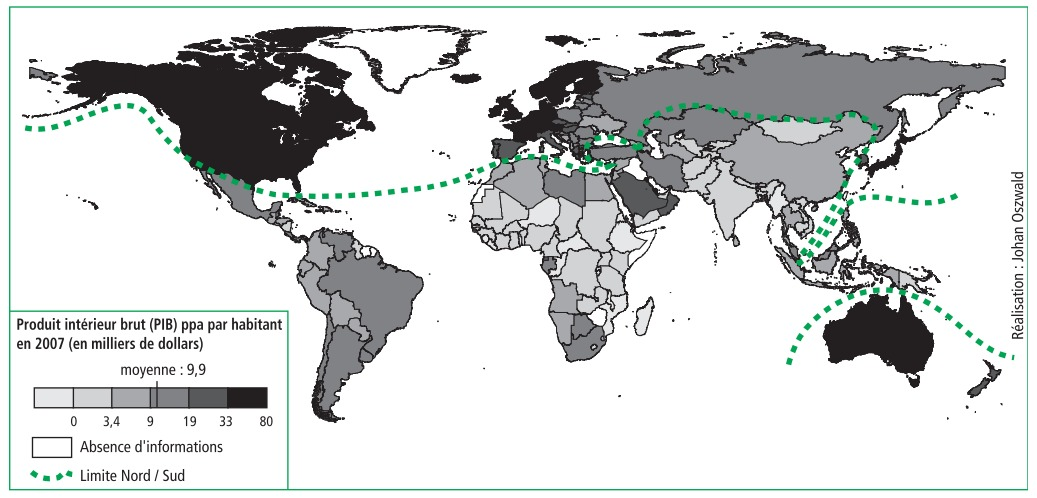
\includegraphics[height=5.5cm]{images/carte_1_01.jpg}
	\end{center}
	\end{frame}
	
	\begin{frame}
	\frametitle{I -- Des inégalités de développement\\ B -- Des Nord(s) et des Sud(s)}
	\begin{center}
	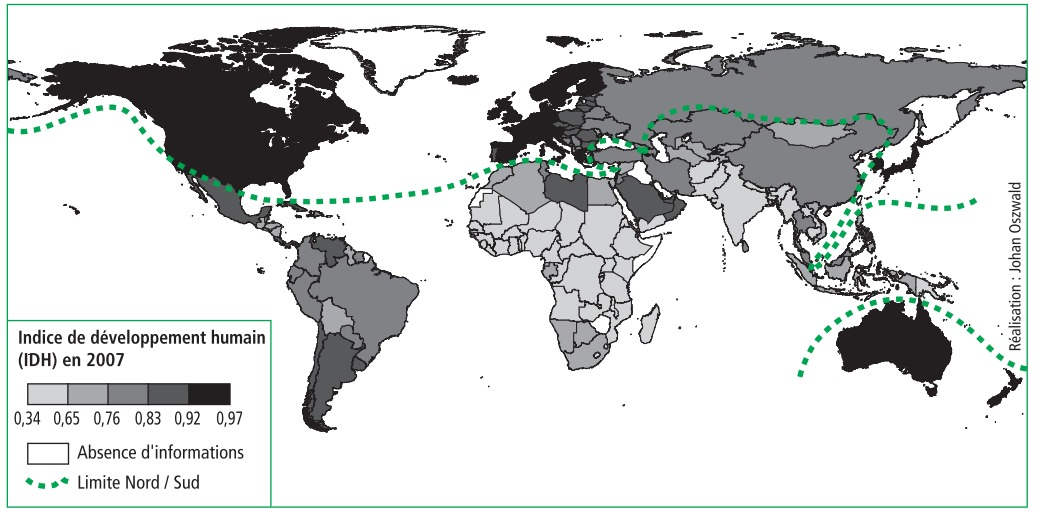
\includegraphics[height=5.5cm]{images/carte_1_02.jpg}
	\end{center}
	\end{frame}
	
	\begin{frame}
	\frametitle{I -- Des inégalités de développement\\ B -- Des Nord(s) et des Sud(s)}
	\begin{itemize}
	\item Les pays riches sont principalement situés dans l'hémisphère nord~: Europe occidentale, Amérique du Nord, Russie, Corée du Sud, Japon, Taïwan, Singapour, Australie, Nouvelle-Zélande. Ces pays sont appelés pays riches, pays industrialisés ou pays du Nord. Ils concentrent 80\% de la richesse mondiale pour 20\% de la population totale.\\
\pause
	\item Les pays pauvres surtout situés dans l'hémisphère sud, en particulier en Afrique et en Asie. La majorité de la population vit du travail de la terre et de l'exploitation des ressources primaires. Ce sont les pays du Sud.
	\end{itemize}
=> Les écarts de richesse entre les 2 groupes de pays tendent à se creuser
	\end{frame}
	
	\begin{frame}
	\frametitle{I -- Des inégalités de développement\\ B -- Des Nord(s) et des Sud(s)}
	\begin{itemize}
	\item On peut noter que des pays qui ont un bon niveau de richesse peuvent avoir un IDH inférieur à la moyenne~: Arabie Saoudite, Brésil, Afrique du Sud\\
\pause
	\item A l'inverse, des pays comme la Bolivie, le Paraguay ou le Mexique ont un PIB assez faible, mais un IDH supérieur à la moyenne mondiale.
	\end{itemize}
=> \textbf{La croissance économique et le développement sont 2 choses différentes.}
\\
L'exemple chinois à travers un article de la revue \textit{Le Point}. Le PIB est un indicateur qu'il faut nuancer.
	\end{frame}
	
	\begin{frame}
	\frametitle{I -- Des inégalités de développement\s\ B -- Des Nord(s) et des Sud(s)}
	\href{run:ArticlePoint.pdf}{«~Chine~: deuxième économie, 150 millions de pauvres~»}, \textit{LePoint.fr}, 15/02/2011.\\
\pause
	\begin{center}
	\textbf{En quoi la richesse globale de la Chine n'est pas représentative de la richesse des individus vivants dans ce pays~?}
	\end{center}
	\end{frame}
	
	\subsection*{TP -- \'Etude de cas~: Le Kenya}
	\begin{frame}
	\frametitle{TP -- \'Etude de cas~: Le Kenya}
	\begin{center}
	\textbf{Problématique~:} Comment se manifestent les inégalités de développement au Kenya~?
	\end{center}
	\end{frame}
	
	\begin{frame}
	\frametitle{TP -- \'Etude de cas~: Le Kenya}
	\textbf{1 -- La croissance du Kenya lui a-t-elle permis d'accéder pour l'instant au développement~?}\\
\pause
La croissance économique du Kenya ne lui a pas permis d'accéder au développement. Certes, cette croissance est relativement soutenue (14,1\%), mais les autres indicateurs montrent que la pauvreté est encore importante (IPM), que l'éducation n'est pas encore accessible à tous (alphabétisation des femmes est faible), et que l'accès aux soins n'est pas encore généralisé (0,14 médecin pour 100 hab.), ce dont rend aussi compte l'important taux de mortalité infantile.
\textbf{-> L'IDH, enfin, montre que si le Kenya est un pays où le développement économique est réel, le développement humain lui est encore à venir.}
	\end{frame}
	
	\begin{frame}
	\frametitle{ TP -- \'Etude de cas~: Le Kenya}
	\textbf{2 -- Quelles inégalités montre le Doc 4~? Donnez-en des facteurs explicatifs à l'aide des Doc 1 et 5.}\\
\pause
Le doc 4 montre de très fortes inégalités régionales puisque le nord-est compte au moins 3 fois plus de pauvres que la région centrale ou la côte, 2 facteurs d'explications~:
	\begin{itemize}
	\item La présence des \textbf{métropoles de Nairobi et de Mombassa} qui produisent l'essentiel des richesses du pays.\\
\pause
	\item le \textbf{milieu} composé de zones désertiques et donc peu fertiles du désert de Chalbi et de la frontière somalienne.
	\end{itemize}
	\end{frame}
	
	\begin{frame}
	\frametitle{TP -- \'Etude cas de cas~: le Kenya\\ Suite de la réponse à la question 2}
-> cette \textbf{inégalité villes/campagnes} est encore plus visible sur la carte 5 qui montre où sont localisés les principaux foyers producteurs de richesses et de revenus au Kenya. \textbf{La production de richesse, y compris dans un pays agricole}, comme le Kenya, \textbf{se fait très majoritairement en ville.}
\\
\textbf{Cependant}, il n'a pas de corrélation automatique entre productions de richesses urbaines et faiblesses du taux de pauvreté régional (ex~: taux de pauvreté aussi élevé entre Nyanza et \textit{rift valley} alors que cette dernière produit moins de richesses).
	\end{frame}
	
	\begin{frame}
	\frametitle{TP -- \'Etude de cas~: le Kenya}
	\begin{center}
	\textbf{3 -- Analysez les inégalités de développement entre villes et campagnes. Doc 3}
	\end{center}
Le doc.3 montre les variations des indicateurs de pauvreté entre les villes et les campagnes au Kenya. Ce pays reste majoritairement rural et, de ce fait, les moyennes nationales sont plus proches des chiffres ruraux.\\
\pause
Pour tous les indicateurs, la pauvreté est moins marquée en ville qu'à la campagne. Le doc permet de se rendre compte du niveau de développement au Kenya~: les \textbf{écarts sont faibles} en ce qui concerne les indicateurs relevant de grandes politiques nationales (\textbf{éducation, santé, etc.} alors qu'ils sont \textbf{plus importants} concernant les autres indicateurs (\textbf{logement, accès aux services en réseaux, etc.;}\\
\pause
\textbf{-> L'inégalité ville/campagne se retrouve assez nettement sur le doc.4 et explique les inégalités régionales.}
	\end{frame}
	
	\begin{frame}
	\frametitle{TP -- \'Etude de cas~: le Kenya}
	\begin{center}
	\textbf{Montrez que les espaces urbains présentent de fortes inégalités sociales, mais aussi spatiales. Doc 6 et 7.}\\
\pause
	\end{center}
Les villes apparaissent moins pauvres que les campagnes, la pauvreté et les disparités socio-économiques y sont cependant très fortes. Les deux documents portent sur la question du logement. Le texte revient sur la question de l'identification des \textbf{classes moyennes et sur le fait qu'une partie de cette catégorie subit aussi une certaine forme exclusion et à recours aux formes d'habitat informel.} La photo montre l'un des bidonvilles les plus connus de Nairobi, Kibera, dominé au dernier plan par des immeubles de standing~: sécurisés, aménagés où des services publics pour la récupération des déchets ou l'accès aux crèches sont mis en place. Dorénavant, on trouve des b\^atiments en dur dans les bidonvilles, particulièrement au premier plan de la photo.
	\end{frame}
	
	\begin{frame}
	\frametitle{TP -- \'Etude de cas~: le Kenya\\ fin de la question 4}
\textbf{-> on remarque la présence d'un habitat spontané ou informel (bidonvilles) qui s'oppose aux \textit{compounds} (immeubles protégés abritant des populations aisées)~: des frontières «~électrifiées~» séparent les quartiers riches du reste de la ville.}
	\end{frame}
	
	\subsection*{C -- L'envers du développement}
	\begin{frame}
	\frametitle{C -- L'envers du développement}
	\begin{center}
	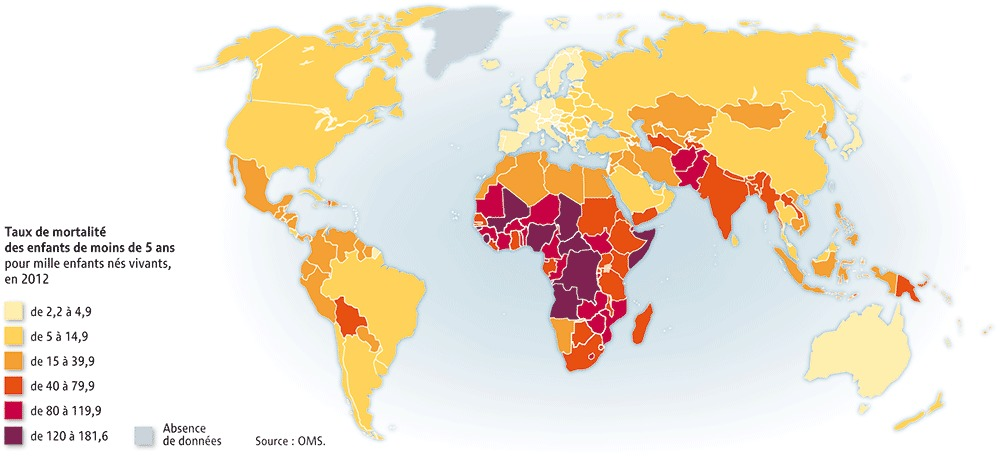
\includegraphics[height=5cm]{images/carte_1_04.jpg}
	\end{center}
Carte~: «~taux de mortalité avant l'âge de 5 ans~»
\\
Où la mortalité infantile est-elle la plus forte~?	
	\end{frame}
	
	\begin{frame}
	\frametitle{C -- L'envers du développement}
	\begin{itemize}
	\item Mortalité infantile forte dans les pays d'Afrique subsaharienne (Niger, Tchad, Congo, etc.), Afghanistan, Irak, Asie du Sud (Inde, Bangladesh, Pakistan, Birmanie, etc.)
	\end{itemize}
	\end{frame}
	
	\begin{frame}
	\frametitle{C -- L'envers du développement}
	\begin{center}
	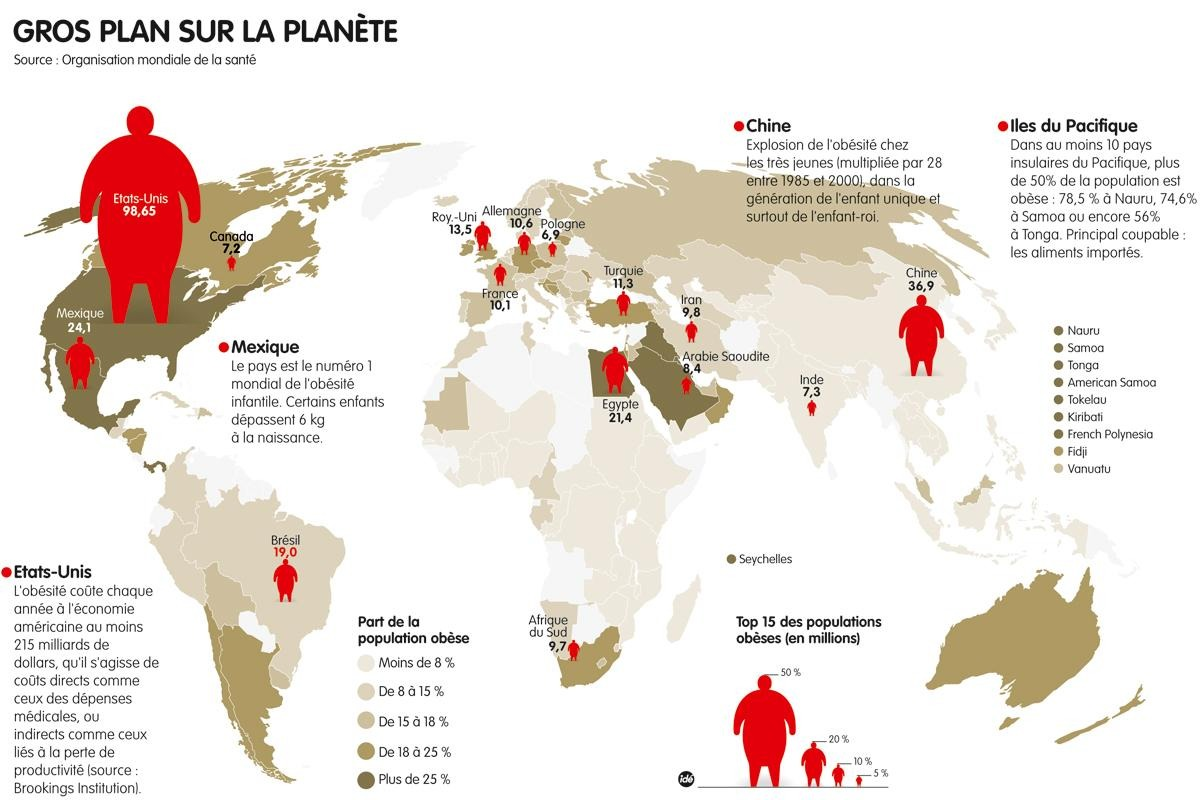
\includegraphics[height=5.5cm]{images/carte_1_05.jpg}
	\end{center}
\\
Carte~:«~gros plan sur la planète~~»
\\
Dans quels pays le nombre d'obèses est le plus fort~?
	\end{frame}
	
	\begin{frame}
	\frametitle{C -- L'envers du développement}
	\begin{itemize}
	\item Les pays où le nombre d'obèses est le plus important sont situés principalement dans le Nord économique (\'Etats-Unis, Australie), Arabie Saoudite, \'Egypte et Argentine.
	\end{itemize}
	\end{frame}
	
	\begin{frame}
	\frametitle{C -- L'envers du développement}
	\begin{center}
	\textbf{Que constate-t-on en regardant ces deux cartes~?}
	\end{center}
	\begin{enumerate}
	\item On constate qu'il y a une inégale répartition des productions~: la nourriture est suffisante, mais inégalement répartie
	\item On constate également que l'obésité, considérée comme un des excès du développement dû à une surconsommation dans les sociétés riches (\'Etats-Unis) s'étend rapidement dans les pays du Sud (comme la Chine par exemple).
	\end{enumerate}
	\end{frame}
	
	\begin{frame}
	\frametitle{C -- L'envers du développement}
	\begin{center}
	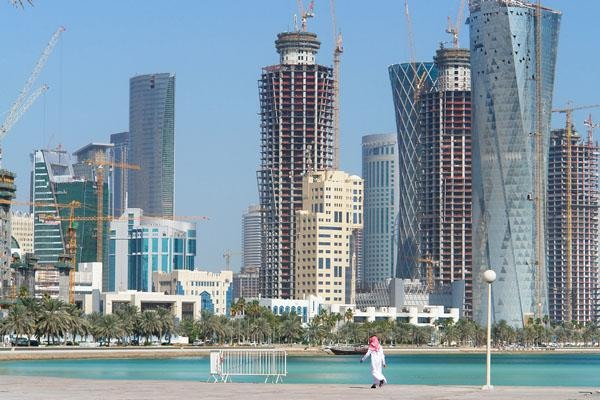
\includegraphics[height=2cm]{images/carte_1_06.jpg}
	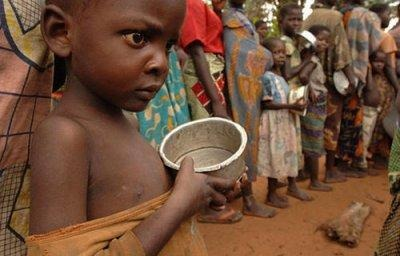
\includegraphics[height=2cm]{images/carte_1_07.jpg}
	\end{center}
	\begin{center}
	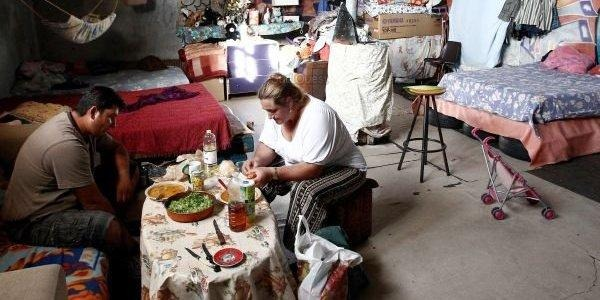
\includegraphics[height=2cm]{images/carte_1_08.jpg}
	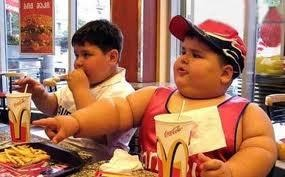
\includegraphics[height=2cm]{images/carte_1_09.jpg}
	\end{center}
	\end{frame}

	\section*{II -- De nouveaux besoins pour une humanité de plus de 9 milliards en 2050}
	\subsection*{TP -- L'Inde~: comment faire face aux besoins d'1,6 milliard d'habitants en 2050~?}
	\begin{frame}{II -- TP -- L'Inde~: comment faire face aux besoins d'1,6 milliard d'habitants en 2050~?}
	\textbf{1 -- Pourquoi la croissance de la population a-t-elle été aussi forte des années 1915 à 2013~? Le rythme de la croissance va-t-il \^etre aussi élevé ensuite~? Quelles sont les prévisions pour 2050~?} (doc. 3)\\
\pause
Le doc 3 correspond au schéma de la transition démographique en Inde entre 1901 et 2050. La période entre 1950 et 2013 correspond à la phase maximale de l'accroissement naturel. En d'autres termes, dans cette phase, on constate d'un taux de natalité d'élevé et un taux mortalité en baisse. \'À l'horizon 2030, la croissance démographique de l'Inde devrait entrer dans un nouveau régime où les taux de natalité et de mortalité seront bas ce qui devrait, naturellement, entraîner une stabilisation de la croissance démographique indienne.
	\end{frame}
	
	\begin{frame}{II -- TP -- L'Inde~: comment faire face aux besoins de1,6 milliard d'habitants en 2050~?}
	\begin{center}
	\includegraphics[height=5.5cm]{images/image5.jpg}
	\end{center}
	
	\end{frame}		
	
	\begin{frame}{II -- TP -- L'Inde~: comment faire face aux besoins de1,6 milliard d'habitants en 2050~?}
	\textbf{2 -- Quelles sont les régions très densément peuplées~? Sont-elles encore en forte croissance démographique~?} (doc 1 et 2)\\
\pause
	Les régions très densément peuplées se situent dans le nord du pays comme le montre le doc 1 «~Densité de population et croissance démographique en Inde~». Comme nous pouvons le lire dans le document 2, «~[...] la transition démographique est achevée dans un grand nombre d'\'Etats en particulier dans l'Inde du Sud, elle est toujours en cours voir relativement peu avancée dans certains \'Etats du nord du pays parmi lesquels figurent des \'Etats très peuplés.~». Par conséquent, les provinces du nord de l'Inde connaissent une forte croissance démographique du fait qu'elles n'ont pas encore achevé leur transition démographique.
	\end{frame}
	
	\begin{frame}{II -- TP -- L'Inde~: comment faire face aux besoins de1,6 milliard d'habitants en 2050~?}
	\textbf{3 -- Par quels moyens l'Inde parvient-elle à ralentir la croissance démographique~? (doc 5) \`A quelle conséquence négative de la politique antinaliste l'Inde doit-elle faire face~? (doc 2)}\\
\pause
L'Inde parvient à ralentir sa croissance démographique en diffusant massivement des moyens de contraception. Le doc. 5 est une affiche «~incitant les couples à utiliser un moyen de contraception~». Depuis les années 1980, l'Inde développe une politique antinatliste incitative qui repose sur le planning familial et sur l'éducation des filles. Toutefois, cette politique n'est pas sans poser des problèmes pour les générations à venir. Par tradition, les familles préfèrent avoir un garçon comme enfant unique qu'une fille. Par conséquent, il existe un fort déséquilibre entre le nombre de garçons et de fille. 
	\end{frame}
	
	\begin{frame}{II -- TP -- L'Inde~: comment faire face aux besoins de1,6 milliard d'habitants en 2050~?}
	\textbf{question 3 suite et fin~:}
\\
Dans le doc. 2, on peut lire, «~Au Punjab où la masculinité dépassait 125 garçons pour 100 filles en 2001 chez les 0-6 ans, il semble qu'elle ne soit plus que de 118  en 2011.~» Cette situation provoque des violences au sein de cette région où le nombre de garçons est bien supérieur à celui des filles.
	\end{frame}
	
	\begin{frame}{II -- TP -- L'Inde~: comment faire face aux besoins de1,6 milliard d'habitants en 2050~?}
\textbf{4 -- Dans quels domaines les besoins de la population vont-ils augmenter~?}(doc.4 et 6)\\
\pause
Les besoins de la population vont augmenter au niveau des besoins élémentaires comme l'accès à l'eau, la lutte contre la pauvreté, l'accès à l'éducation et au soin. Le pays conna\^it déjà un «~stress hydrique~» c'est-à-dire que la demande en eau est supérieure aux ressources. \`A l'échelle d'un pays, on mesure le plus souvent l'accès à l'eau douce, en évaluant la quantité d'eau douce par habitant et par an. On parle de stress hydrique, lorsque ces ressources sont inférieures à 1700m3 par habitant et par an, et de pénurie,lorsqu'elles sont inférieures à 1000m3/hab/an. La ressource en eau est inégale dans le pays et souvent s'ajoute de graves problèmes de pollution. 
	\end{frame}
	
	\begin{frame}{II -- TP -- L'Inde~: comment faire face aux besoins de1,6 milliard d'habitants en 2050~?}
\textbf{question 4 suite et fin}
\\
On peut donc se demander comme l'Inde pourra faire face aux besoins en eau d'une population en perpétuelle augmentation. Enfin, en raison des grandes inégalités existantes déjà à l'intérieur du pays, il est nécessaire que le pays puisse développer un plan de lutte contre la pauvreté afin d'éviter un exode des populations vers les grands urbains déjà saturés. Pour ce faire, l'Inde peut éventuellement réfléchir à une relance du secteur agricole.
Enfin, l'Inde doit moderniser son pays au niveau de l'accès au soin et à l'éducation afin de permettre à chacun de profiter d'une possible promotion sociale par et gr\^ace à l'école.
	\end{frame}
	
	\begin{frame}{II -- TP -- L'Inde~: comment faire face aux besoins de1,6 milliard d'habitants en 2050~?}
\textbf{5 -- Quels défis l'Inde doit-elle encore surmonter pour que sa croissance économique se transforme en véritable développement~?} (doc 2, 4 et 6)\\
\pause
Inde doit surmonter le défi de l'alphabétisation et notamment celle des femmes pour que sa croissance économique se transforme en véritable développement. Il faudrait également qu'elle dépasse des problèmes environnementaux liés notamment à l'accès et à la pollution de l'eau. Enfin, l'Inde doit progresser en termes d'accès au soin et de lutte contre la pauvreté afin que sa forte croissance économique puisse profiter aux populations les moins favorisées.
	\end{frame}
	
	\subsection*{A -- la croissance de la population mondiale}
	\begin{frame}{A -- la croissance de la population mondiale}
	\begin{center}
	\textbf{Observez les graphiques suivants et donnez pour chacun d'eux le type d'évolution qu'il prévoit pour la planète en 2050}
	\end{center}
	\end{frame}
	
	\begin{frame}{A -- la croissance de la population mondiale}
	\begin{center}
	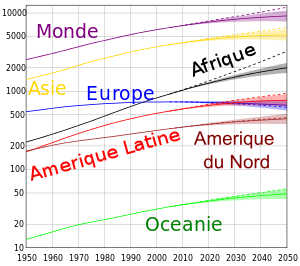
\includegraphics[height=5.5cm]{images/image1.png}
	\end{center}
	Doc. 1. \'Evolution de la population mondiale par continent jusqu'en 2050
	\end{frame}
	
	\begin{frame}{A -- la croissance de la population mondiale}
	\textbf{Croissance de la population}~: on passera théoriquement de 7 milliards aujourd'hui à 9,2 milliards en 2050 selon ce graphique, car la \textbf{transition démographique} des pays du Sud n'est pas encore achevée. L'augmentation de la population mondiale est essentiellement liée à ces pays.
	\end{frame}
	
	\begin{frame}{A -- la croissance de la population mondiale}
	\begin{center}
	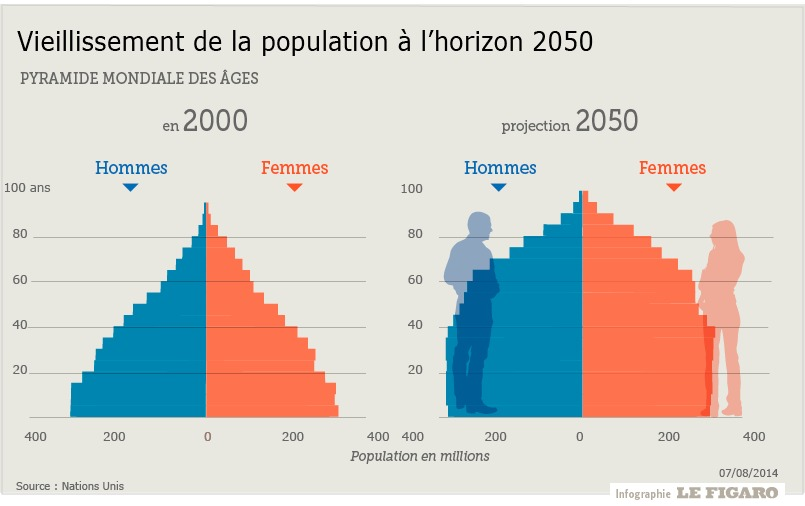
\includegraphics[height=5.5cm]{images/carte_1_12.jpg}
	\end{center}
	Doc. 2 Vieillissement de la population à l'horizon 2050
	\end{frame}
	
	\begin{frame}{A -- la croissance de la population mondiale}
	L'espérance de vie à la naissance devrait dépasser les 75 ans. C'est le \textbf{vieillissement démographique} (allongement de la durée de vie, familles moins nombreuses. Le pourcentage de personnes de plus de 65 ans devrait doubler par rapport à aujourd'hui.
	\end{frame}
		
	\begin{frame}{A -- la croissance de la population mondiale}
	\begin{center}
	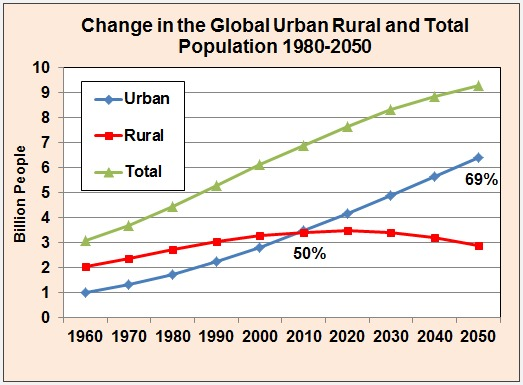
\includegraphics[height=5.5cm]{images/carte_1_13.jpg}
	\end{center}
	Doc. 3 Répartitions de la population entre les espaces rural et urbain jusqu'en 2050
	\end{frame}
	
	\begin{frame}{A -- La croissance de la population mondiale}
	aujourd'hui 50\% de la population mondiale vit en ville, on estime à 69\% en 2050.
	\end{frame}
	
	\subsection*{B -- Quels besoins pour 2050~?}
	\begin{frame}{Quels besoins pour 2050~?}
	\begin{itemize}
	\item Aujourd'hui, 3 milliards d'hommes n'ont pas accès aux besoins élémentaires~: santé, éducation, nourriture. Ils sont vulnérables face aux \textbf{pandémies} (épidémies qui s'étendent sur plusieurs continents et sur une longue durée) et aux risques naturels\.\
\pause
	.\item Entre 1980 et 2005, le nombre de très pauvres dans le monde a diminué de moitié (25\% à 26\%). La croissance économique chinoise et le programme «~faim zéro~» au Brésil ont permis d'aller dans ce sens. Au contraire, en Afrique, la pauvreté gagne encore du terrain, elle a doublé sur la m\^eme période.\\
\pause
	\item Qu'en sera-t-il en 2050~? Les besoins agricoles pourraient demander un doublement de la production mondiale. Les besoins en ressources minières et en énergies fossiles créeront encore plus de tensions géopolitiques.
	\end{itemize}
	\end{frame}
	
	\section*{III -- Vers des modes durables de développement~?}
	\begin{frame}
	\frametitle{III -- Vers des modes durables de développement~?}
	\end{frame}
	
	\subsection*{TP -- Vidéo «~Présentation de l'entreprise ENVIE Toulouse/Montauban~»}
	\begin{frame}{TP -- Vidéo «~Présentation de l'entreprise ENVIE Toulouse/Montauban~»}
	\href{http://www.envie-midipyrenees.com/les-dix-ans-denvie-toulouse/}{«~30 mars 2010~: Les dix ans d'Envie Toulouse~» vidéo de TLT (Chaîne de télévision locale toulousaine)}
	\end{frame}
	
	\begin{frame}{TP -- Vidéo «~Présentation de l'entreprise ENVIE Toulouse/Montauban~»}
	\begin{center}
	\textbf{Compléter le tableau ci-dessous}
	\end{center}
	\begin{tabular}{|c|c|}
	\hline
L'écologie & comment l'entreprise participe-t-elle \\ & à la protection de la nature ? \\
	\hline
L'économie & comment l'entreprise permet-elle\\ & aux ménages d'éviter le surendettement ?\\
	\hline
Le social & comment l'entreprise participe-t-elle\\ & à l'amélioration des conditions de vie de la population~?\\
	\hline
	\end{tabular}
	\end{frame}	
	
	\begin{frame}{TP -- Vidéo «~Présentation de l'entreprise ENVIE Toulouse/Montauban~»}
	\begin{itemize}
	\item \textbf{Le social}~: Comment l'entreprise participe-t-elle à l'amélioration des conditions de vie de la population~?\\
\pause
		\begin{itemize}
		\item L'entreprise repose sur l'\textbf{insertion} des personnes en difficultés~: demandeurs d'emploi, au RSA, etc. L'objectif de leur permettre d'obtenir un contrat d'insertion de deux ans avec un accompagnement professionnel afin de retourner dans la vie active à trouvant un nouvel emploi
		\end{itemize}
	\end{itemize}
	\end{frame}
	
	\begin{frame}{TP -- Vidéo «~Présentation de l'entreprise ENVIE Toulouse/Montauban~»}
	\begin{itemize}
	\item \textbf{L'économie}~: Comment l'entreprise permet-elle aux ménages d'éviter le surendettement~?
		\begin{itemize}
		\item L'entreprise Envie possède une activité commerciale qui permet à toutes personnes de pouvoir acheter du matériel électroménager d'occasion avec une garantie. Cela offre l'opportunité aux personnes dans le besoin de pouvoir acquérir ces biens sans passer des crédits à la consommation et sans entrer, éventuellement, dans la spirale du surendettement.
		\end{itemize}
	\end{itemize}
	\end{frame}
	
	\begin{frame}{TP -- Vidéo «~Présentation de l'entreprise ENVIE Toulouse/Montauban~»}
	\begin{itemize}
	\item \textbf{L'écologie}~: Comment l'entreprise participe-t-elle à la protection de la nature~?
		\begin{itemize}
		\item \textbf{Recycler}~: traiter des déchets pour qu'ils reviennent dans le cycle de production (ex du verre)
		\item \textbf{Reconditionner}~: Remettre en condition de marche
		\item \textbf{Dépolluer}~: enlever les matières nocives (batteries, gaz de refroidissement)
		\item \textbf{Démanteler}~: déconstruction des éléments (séparer le plastique du métal, l'électronique du mécanique, etc.)
		\end{itemize}
	\end{itemize}
	\end{frame}
	
	
	\subsection*{A -- qu'est-ce que le développement durable}
	\begin{frame}{Qu'est-ce que le développement durable}
	\textbf{Rappel}~: Nous l'avons vu dans l'introduction, le rapport Brundtland de 1987 définit le développement durable comme «~\textbf{le développement qui répond aux besoins des générations actuelles sans compromettre la capacité des générations futures à répondre aux leurs}\\
	Il repose sur 3 piliers~:
	\begin{center}
	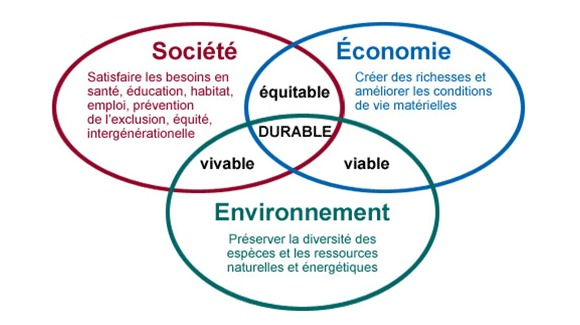
\includegraphics[height=3cm]{images/carte_1_16.jpg}
	\end{center}
	\end{frame}
	
	\subsection*{B -- Du développement durable aux développements durables}
	\subsubsection*{1) une mise en œuvre difficile}
	\begin{frame}{B -- Du développement durable aux développements durables\\ 1) une mise en œuvre difficile}
	\begin{center}
	\textbf{Lecture des documents et réponses aux questions de la page 29}
	\end{center}
	\end{frame}
	
	\begin{frame}{B -- Du développement durable aux développements durables\\ 1) une mise en œuvre difficile}
	\textbf{\`A quels piliers du développement durable se rattachent les Objectifs du développement durable~?}
	\begin{itemize}
	\item Pilier social~: éliminer l'extrême pauvreté (1), assurer l'éducation primaire pour tous (2), promouvoir l'égalité et l'autonomisation des femmes (3), réduire la mortalité infantile (4), améliorer la santé maternelle (5), combattre le VIH/Sida, le paludisme et d'autres maladies (6)\\
\pause
	\item Pilier environnemental~: assurer un environnement stable (7)\\
\pause
	\item Pilier économique~: mettre en place un partenariat mondial pour le développement (8)
	\end{itemize}
	\end{frame}
	
		\begin{frame}[allowframebreaks]{B -- Du développement durable aux développements durables\\ 1) une mise en œuvre difficile}
		\textbf{Analyser le message de l'ADEME et la façon dont il est transmis}\\
La brochure s'intitule \textit{Le développement durable} avec comme sous-titre  «~Pour tous, grâce à tous, au présent et au futur~». Ici L'ADEME (Agence de l'Environnement et de la Maîtrise de l'\'Energie) étudie tout particulièrement la question des énergies sous l'angle du développement durable. L'illustration de la couverture montre plusieurs générations, un vieux monsieur à droite, mais surtout deux enfants l'un qui représente les pays du Nord puisqu'il est assis sur l'hémisphère Nord du globe et un second qui représente par sa position les pays du Sud. l'ADEME indique ainsi que la question énergétique concerne les générations actuelles, mais aussi et surtout les générations futures sans exclusions d'origine. La lutte contre le réchauffement climatique concerne les pays du Nord comme du Sud et les mesures doivent être prises par tous les pays à la hauteur de leurs possibilités économiques, sociales et environnementales.
		\end{frame}
		
		\begin{frame}{B -- Du développement durable aux développements durables\\ 1) une mise en œuvre difficile}
		\textbf{Quelles sont les contradictions et les difficultés de mise en œuvre du développement durable pointées par le document 3}\\
Il faut nécessairement permettre aux habitants de pays du Sud d'accéder au niveau de développement des pays du Nord. Toutefois, si l'ensemble de la population devait utiliser les modes de déplacement des Américains, la pollution serait très forte et les ressources en pétrole seraient très vite épuisées. Il faut donc permettre aux populations des pays émergents de pouvoir accéder au développement sans que cela nuise d'un point de vue environnemental, social ou économique au reste du monde.
		\end{frame}
		
		\subsubsection*{2) Des modes durables de développement}
		\begin{frame}{B -- Du développement durable aux développements durables\\ 2) des modes durables de développement}
		\textbf{L'application des piliers du développement durable (DD)} est surtout dans les pays riches, notamment des pays de l'UE (cf. carte 4, p.37) : PAC, Natura 2000 (sites naturels), gestion des risques, développement de l'agriculture durable, Agenda 21 (aménagement durable de la ville)
		\end{frame}
		
		\begin{frame}{B -- Du développement durable aux développements durables\\ 2) des modes durables de développement}
		\begin{center}
		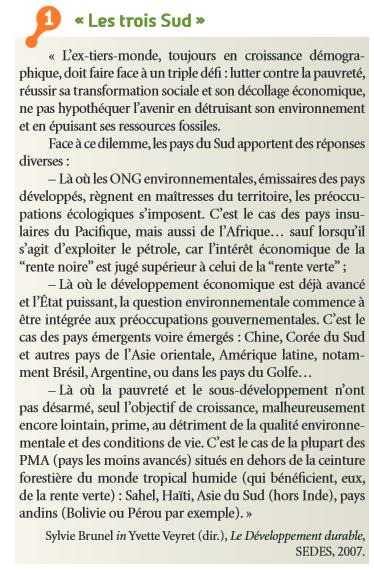
\includegraphics[height=5.5cm]{images/carte_1_18.jpg}
		\end{center}
		\end{frame}
	
	\section*{Conclusion}
	\begin{frame}
	\frametitle{Conclusion}
	Le DD est difficile à mettre en oeuvre à l'échelle mondiale. On distingue des oppositions entre Nord/Sud entre les Nords et les Suds, villes/campagnes.\\
	Le DD n'est pas une solution, il faut mettre en place \textbf{des modes durables de développement} où l'homme utilise et respecte les rapports en nature et société.
	\end{frame}
\end{document}